\documentclass{article}
\title{SML Uebung 1}
\author{Yi Cui , Lingwei liu}
\usepackage{amsmath}
\usepackage{ulem}
\usepackage{arydshln}
\usepackage{amsfonts}
\usepackage{listings}
\usepackage{color}
\usepackage{geometry}
\usepackage{graphicx} 
\usepackage{float} 
\usepackage{subfigure} 
\geometry{left=3cm,right=3cm,top=3cm,bottom=3cm}


\definecolor{dkgreen}{rgb}{0,0.6,0}
\definecolor{gray}{rgb}{0.5,0.5,0.5}
\definecolor{mauve}{rgb}{0.58,0,0.82}

\lstset{frame=tb,
  language=Python,
  aboveskip=3mm,
  belowskip=3mm,
  showstringspaces=false,
  columns=flexible,
  basicstyle={\small\ttfamily},
  numbers=none,
  numberstyle=\tiny\color{gray},
  keywordstyle=\color{blue},
  commentstyle=\color{dkgreen},
  stringstyle=\color{mauve},
  breaklines=true,
  breakatwhitespace=true,
  tabsize=3
}
\begin{document}
\maketitle
\newpage
\section* {Task 1}
%--------------------------------------------------------------------------------------------------1a---------------------------------------------------------------------------------------
\subsection*{1a}
\uuline{A}=
$
\begin{bmatrix} 
a_{11}&a_{12}&\cdots&a_{1n}\\
a_{21}&\ddots& &a_{2n}\\
\vdots& & &\vdots\\
a_{n1}&\cdots& &a_{nn}
\end{bmatrix} 
\quad
$
\uuline{B}=
$
\begin{bmatrix} 
b_{11}&b_{12}&\cdots&b_{1n}\\
b_{21}&\ddots& &b_{2n}\\
\vdots& & &\vdots\\
b_{n1}&\cdots& &b_{nn}
\end{bmatrix} 
\quad
$
\uuline{C}=
$
\begin{bmatrix} 
c_{11}&c_{12}&\cdots&c_{1n}\\
c_{21}&\ddots& &c_{2n}\\
\vdots& & &\vdots\\
c_{n1}&\cdots& &c_{nn}
\end{bmatrix} 
\quad
$
\\[15pt]
%------------------------------------------------------------------------------------------------1a结合律--------------------------------------------------------------------------------
associative:
%-------------------------------------------------------------------------------------------------(AB)C--------------------------------------------------------------------------------
\begin{equation}\notag
\begin{aligned}
( \uuline{A}\cdot\uuline{B} ) \uuline{C} &= 
\begin{bmatrix} 
\sum\limits_{i=1}^{n} a_{1i}b_{i1}&\cdots& \sum\limits_{i=1}^{n} a_{1i}b_{in}\\
\vdots&\ddots&\vdots\\
\sum\limits_{i=1}^{n} a_{ni}b_{i1}&\cdots& \sum\limits_{i=1}^{n} a_{ni}b_{in}
\end{bmatrix} 
\quad
\cdot
\begin{bmatrix}
c_{11}&\cdots&c_{1n}\\
\vdots&\ddots&\vdots\\
c_{n1}&\cdots&c_{nn}
\end{bmatrix} 
\quad
\\[15pt]
&= 
\begin{bmatrix} 
\sum\limits_{j=1}^{n}(\sum\limits_{i=1}^{n} a_{1i}b_{ij})\cdot c_{j1}&\cdots& \sum\limits_{j=1}^{n} (\sum\limits_{i=1}^{n} a_{1i}b_{ij})\cdot c_{jn}\\
\vdots&\ddots&\vdots\\
\sum\limits_{j=1}^{n}(\sum\limits_{i=1}^{n} a_{ni}b_{ij})\cdot c_{j1}&\cdots& \sum\limits_{j=1}^{n}(\sum\limits_{i=1}^{n} a_{ni}b_{ij})\cdot c_{jn}
\end{bmatrix} 
\quad
\end{aligned}
\end{equation}
%-------------------------------------------------------------------------------------------------A(BC)------------------------------------------------------------------------------------
\begin{equation}\notag
\begin{aligned}
\uuline{A}( \uuline{B}\cdot\uuline{C} ) &= 
\begin{bmatrix}
a_{11}&\cdots&a_{1n}\\
\vdots&\ddots&\vdots\\
a_{n1}&\cdots&a_{nn}
\end{bmatrix} 
\quad
\cdot
\begin{bmatrix} 
\sum\limits_{i=1}^{n} b_{1i}c_{i1}&\cdots& \sum\limits_{i=1}^{n} b_{1i}c_{in}\\
\vdots&\ddots&\vdots\\
\sum\limits_{i=1}^{n} b_{ni}c_{i1}&\cdots& \sum\limits_{i=1}^{n} b_{ni}c_{in}
\end{bmatrix} 
\quad
\\[15pt]
&= 
\begin{bmatrix} 
\sum\limits_{j=1}^{n}a_{1j}\cdot(\sum\limits_{i=1}^{n} b_{ji}c_{i1})&\cdots& \sum\limits_{j=1}^{n}a_{1j}\cdot(\sum\limits_{i=1}^{n} b_{ji}c_{in})\\
\vdots&\ddots&\vdots\\
\sum\limits_{j=1}^{n}a_{nj}\cdot(\sum\limits_{i=1}^{n} b_{ji}c_{in})&\cdots& \sum\limits_{j=1}^{n}a_{nj}\cdot(\sum\limits_{i=1}^{n} b_{ji}c_{in})
\end{bmatrix} 
\quad
\end{aligned}
\end{equation}
\\[15pt]
element analysis:
\begin{equation}\notag
\begin{aligned}
\sum\limits_{j=1}^{n}(\sum\limits_{i=1}^{n} a_{1i}b_{ij})\cdot c_{j1} &\neq \sum\limits_{j=1}^{n}a_{1j}\cdot(\sum\limits_{i=1}^{n} b_{ji}c_{i1})
\\[15pt]
( \uuline{A}\cdot\uuline{B} ) \uuline{C} &\neq \uuline{A}( \uuline{B}\cdot\uuline{C} )
\\
\end{aligned}
\end{equation}
$\Rightarrow$ associative disproved
%---------------------------------------------------------------------------------------------分配律---------------------------------------------------------------------------------------------
\\[20pt]
distribute:
\begin{equation}\notag
\begin{aligned}
( \uuline{A}+\uuline{B} )\cdot \uuline{C}&=
\begin{bmatrix}
a_{11}+b_{11}&\cdots&a_{1n}+b_{1n}\\
\vdots&\ddots&\vdots\\
a_{n1}+b_{n1}&\cdots&a_{nn}+b_{nn}
\end{bmatrix}
\quad 
\cdot
\begin{bmatrix}
c_{11}&\cdots&c_{1n}\\
\vdots&\ddots&\vdots\\
c_{n1}&\cdots&c_{nn}
\end{bmatrix} 
\quad
\\
&=
\begin{bmatrix} 
\sum\limits_{i=1}^{n}(a_{1i}+b_{1i})\cdot c_{i1}&\cdots& \sum\limits_{i=1}^{n}(a_{1i}+b_{1i})\cdot c_{in}\\
\vdots&\ddots&\vdots\\
\sum\limits_{i=1}^{n}(a_{ni}+b_{ni})\cdot c_{i1}&\cdots& \sum\limits_{i=1}^{n}(a_{ni}+b_{ni})\cdot c_{in}
\end{bmatrix} 
\quad
\\
&=
\begin{bmatrix} 
\sum\limits_{i=1}^{n}a_{1i}\cdot c_{i1}&\cdots& \sum\limits_{i=1}^{n}a_{1i}\cdot c_{in}\\
\vdots&\ddots&\vdots\\
\sum\limits_{i=1}^{n}a_{ni}\cdot c_{i1}&\cdots& \sum\limits_{i=1}^{n}a_{ni}\cdot c_{in}
\end{bmatrix}
+
\begin{bmatrix} 
\sum\limits_{i=1}^{n}b_{1i}\cdot c_{i1}&\cdots& \sum\limits_{i=1}^{n}b_{1i}\cdot c_{in}\\
\vdots&\ddots&\vdots\\
\sum\limits_{i=1}^{n}+b_{ni}\cdot c_{i1}&\cdots& \sum\limits_{i=1}^{n}b_{ni}\cdot c_{in}
\end{bmatrix} 
\\
&=\uuline{A}\cdot \uuline{C}+\uuline{B} \cdot \uuline{C} 
\end{aligned}
\end{equation}
$\Rightarrow$ distribute proved
%--------------------------------------------------------------------------------------------------交换律-----------------------------------------------------------------------------------------
\\[20pt]
commutative:
\begin{equation}\notag
\begin{aligned}
\uuline{A}\cdot\uuline{B} &=
\begin{bmatrix} 
\sum\limits_{i=1}^{n} a_{1i}b_{i1}&\cdots& \sum\limits_{i=1}^{n} a_{1i}b_{in}\\
\vdots&\ddots&\vdots\\
\sum\limits_{i=1}^{n} a_{ni}b_{i1}&\cdots& \sum\limits_{i=1}^{n} a_{ni}b_{in}
\end{bmatrix} 
\quad
\\
\uuline{B}\cdot\uuline{A} &=
\begin{bmatrix} 
\sum\limits_{i=1}^{n} b_{1i}a_{i1}&\cdots& \sum\limits_{i=1}^{n} b_{1i}a_{in}\\
\vdots&\ddots&\vdots\\
\sum\limits_{i=1}^{n} b_{ni}a_{i1}&\cdots& \sum\limits_{i=1}^{n} b_{ni}a_{in}
\end{bmatrix} 
\quad
\end{aligned}
\end{equation}
\\
element analysis:
\begin{equation}\notag
\begin{aligned}
\sum\limits_{i=1}^{n} b_{1i}a_{i1} &\neq \sum\limits_{i=1}^{n} b_{ni}a_{i1}
\\
\uuline{A}\cdot\uuline{B} &\neq \uuline{B}\cdot\uuline{A} 
\end{aligned}
\end{equation}
$\Rightarrow$ commutative disproved
\newpage
%-------------------------------------------------------------------------------------------------1b-----------------------------------------------------------------------------------------------------
\subsection*{1b}
method 1: elementray transformation
\\
%-------------------------------------------------------------------------------------------------method1-------------------------------------------------------------------------------------------------
\begin{equation}\notag
\begin{aligned}
\begin{bmatrix}
\uuline{A}&\uuline{I}
\end{bmatrix} 
&\Longrightarrow
\begin{bmatrix}
\uuline{I}&\uuline{A^{-1}}
\end{bmatrix} 
\quad
\\
\left[ {\begin{array}{c:c}
\begin{matrix}
1&2&3\\
1&4&6\\
0&0&1\\
\end{matrix}&
\begin{matrix}
1&0&0\\
0&1&0\\
0&0&1\\
\end{matrix}
\end{array}} \right]
&\Longrightarrow
\left[ {\begin{array}{c:c}
\begin{matrix}
1&2&3\\
1&0&0\\
0&0&1\\
\end{matrix}&
\begin{matrix}
1&0&0\\
2&-1&0\\
0&0&1\\
\end{matrix}
\end{array}} \right]
\\
\Longrightarrow
\left[ {\begin{array}{c:c}
\begin{matrix}
0&1&0\\
1&0&0\\
0&0&1\\
\end{matrix}&
\begin{matrix}
-\frac{1}{2}&\frac{1}{2}&\frac{3}{2}\\
2&-1&0\\
0&0&1\\
\end{matrix}
\end{array}} \right]
&\Longrightarrow
\left[ {\begin{array}{c:c}
\begin{matrix}
1&0&0\\
0&1&0\\
0&0&1\\
\end{matrix}&
\begin{matrix}
2&-1&0\\
-\frac{1}{2}&\frac{1}{2}&\frac{3}{2}\\
0&0&1\\
\end{matrix}
\end{array}} \right]
\end{aligned}
\end{equation}
\\[20pt]
%-----------------------------------------------------------------------------------------------------method2--------------------------------------------------------------------------------------------
method 2: use adjoint matrix
\begin{equation}\notag
\begin{aligned}
\uuline{A^{-1}}&=
\frac{1}{\lvert A \lvert}
\begin{bmatrix}
A_{11}&\cdots&A_{1n}\\
\vdots&\ddots&\vdots\\
A_{n1}&\cdots&A_{nn}
\end{bmatrix} 
\quad
\Longrightarrow adjoint 
\end{aligned}
\end{equation}
\\[15pt] where $A_{ij}$ is algebraic cofactor
\\[15pt]
\begin{equation}\notag
\begin{aligned}
&=\frac{1}{det(\uuline{A})}\cdot
\begin{bmatrix} 
4&-2&0\\
-1&1&-3\\
0&0&2
\end{bmatrix}
\quad
=
\begin{bmatrix} 
2&-1&0\\
-\frac{1}{2}&\frac{1}{2}&\frac{3}{2}\\
0&0&1\\
\end{bmatrix}
\quad
\\[15pt]
\end{aligned}
\end{equation}
with $det(\uuline{A})=\lvert A \lvert =2$
\\[15pt]
If  $\uuline{A}$ is changed to
$
\begin{bmatrix} 
1&2&3\\
1&4&6\\
1&0&0
\end{bmatrix}
\\[15pt]
det(\uuline{A})=0
\Longrightarrow
$
A is a singular matrix
$\Longrightarrow$ irreversible
\newpage
%----------------------------------------------------------------------------------------------------1c----------------------------------------------------------------------------------------------------
\subsection*{1c}
for $A\in \mathbb{R}^{n\times m} $
\\[15pt]
left Moore-Penrose pseudoinverse:
$
\uuline{A}^f_{left} = (\uuline{A}^T\cdot \uuline{A})^{-1} \cdot \uuline{A}^T
$\\[15pt]
left Moore-Penrose pseudoinverse:
$
\uuline{A}^f_{right} = \uuline{A}^T \cdot (\uuline{A}\cdot \uuline{A}^T)^{-1} 
$\\[15pt]
dimensional analysis:\\[15pt]
if  
$ A\in \mathbb{R}^{2\times 3}$ 
\\
\begin{equation}\notag
\begin{aligned}
\uuline{A}^f_{left} &= (\uuline{A}^T\cdot \uuline{A})^{-1} \cdot \uuline{A}^T
\\
&\Rightarrow (3\times 2)\cdot (2\times 3)\cdot (3\times 2) \Rightarrow (3\times 2)
\\
\uuline{A}^f_{right} &= \uuline{A}^T \cdot (\uuline{A}\cdot \uuline{A}^T)^{-1}
\\
&\Rightarrow (3\times 2)\cdot [(2\times 3)\cdot (3\times 2)] \Rightarrow (3\times 2)
\\
&\Rightarrow \uuline{A}^f \in \mathbb{R}^{2\times 3}
\end{aligned}
\end{equation}
\\[30pt]
%------------------------------------------------------------------------------------------------------1d-----------------------------------------------------------------------------------------------------
\subsection*{1d}
eigenvector: represent the orientation of each principal components\\[15pt]
eigenvalue:  represent the weight of each principal components\\[15pt]
both of them represent the component distribution of all features (PCA perspective)
\newpage
%-------------------------------------------------------------------------------------------------------Task2--------------------------------------------------------------------------------------------
\section*{Task 2}
\subsection*{2a}
%----------------------------------------------------------------------------------------------------------1------------------------------------------------------------------------------------------------
\subsubsection*{1}
for $\Omega$ is a finite set \\[15pt]
Expectation:
\begin{equation}\notag
\begin{aligned} 
E[f(\omega)]=\sum\limits_{\omega \in \Omega} \cdot f(\omega)\cdot P(\omega)
\end{aligned}
\end{equation}
\\[15pt]
Variance:
\begin{equation}\notag
\begin{aligned}
V[f(\omega)] &=\sum\limits_{\omega \in \Omega}P(\omega)\cdot [f(\omega)-E(\omega)]^2
\\
&=E[[f(\omega)-E[f(\omega)]]^2]
\end{aligned}
\end{equation}
\\
For Expection: the rules of  expection prove it:\\
%-----------------------------------------------------------------------------------------不完整要补全
\begin{equation}\notag
\begin{aligned}
E[a\uline{X}] &= aE[\uline{X}]\\
E[\uline{x}+\uline{y}]&= E[\uline{X}]+E[\uline{Y}]\\
E[\sum\limits_{i} a_x x_i]&=
\end{aligned}
\end{equation}
\\
Variance is essential \\
\begin{equation}\notag
\begin{aligned}
V[f(\omega)]&=E[[f(\omega)-E[f(\omega)]]^2]\\
&=E[f(\omega)]^2-2E[f(\omega)]\cdot E[f(\omega)]+(E[f(\omega)])^2\\
&=E[f(\omega)]^2-(E[f(\omega)])^2\\
&=\sum\limits_{\omega \in \Omega}P(\omega) \cdot (f(\omega))^2-E[f(\omega)]^2
\end{aligned}
\end{equation}
\newpage
%------------------------------------------------------------------------------------------------------------2--------------------------------------------------------------------------------------------------
\subsubsection*{2}
For diece A set $P(A)=1 \Rightarrow P(x,A) = P(x|A)\cdot P(A)=P(x|A)=P_A(x)$
\begin{equation}\notag
\begin{aligned} 
\bar x_A = \sum\limits_{i=1}^{6}x_i\cdot P(x_i,A)&=1\cdot 2/9+2\cdot 1/18 +3\cdot 1/3 + 4\cdot 1/9 +5\cdot 1/18 +6\cdot 2/9\\
&= 61/18 \approx 3.3889
\\
unbiased \quad V[(x,A)]&=\frac{1}{N-1}  \cdot  = \sum\limits_{i=1}^{N=18}(X_i-\bar X_A)^2 \qquad (Bessel's Correction)\\
&=\frac{1}{17}\cdot (4\cdot(1-\frac{61}{18})^2+1\cdot(2-\frac{61}{18})^2+6\cdot(3-\frac{61}{18})^2+2\cdot(4-\frac{61}{18})^2
\\&+1\cdot(5-\frac{61}{18})^2+4\cdot(6-\frac{61}{18})^2)\\
&=\frac{1013}{306}  \approx 3.3105
\end{aligned}
\end{equation}
\\[15pt]
For diece B set $P(B)=1 \Rightarrow P(x,B) = P(x|B)\cdot P(B)=P(x|B)=P_B(x)$
\begin{equation}\notag
\begin{aligned} 
\bar x_B = \sum\limits_{i=1}^{6}x_i\cdot P(x_i,B)&=1\cdot 5/18+2\cdot 1/3 +3\cdot 1/18 + 4\cdot 1/18 +5\cdot 2/9 +6\cdot 1/18\\
&= 25/9 \approx 2.7778
\\
unbiased \quad V[(x,B)]&=\frac{1}{N-1}  \cdot  = \sum\limits_{i=1}^{N=18}(X_i-\bar X_B)^2 \qquad \\
&=\frac{1}{17}\cdot (5\cdot(1-\frac{25}{9})^2+6\cdot(2-\frac{25}{9})^2+1\cdot(3-\frac{25}{9})^2+1\cdot(4-\frac{25}{9})^2
\\&+4\cdot(5-\frac{25}{9})^2+1\cdot(6-\frac{25}{9})^2)\\
&=\frac{460}{153}  \approx 3.0065
\end{aligned}
\end{equation}
\\[15pt]
For diece C set $P(C)=1 \Rightarrow P(x,C) = P(x|C)\cdot P(C)=P(x|C)=P_C(x)$
\begin{equation}\notag
\begin{aligned} 
\bar x_C = \sum\limits_{i=1}^{6}x_i\cdot P(x_i,C)&=1\cdot 1/6+2\cdot 1/6 +3\cdot 2/9 + 4\cdot 1/9 +5\cdot 1/6 +6\cdot 1/6\\
&=31/9 \approx 3.4444
\\
unbiased \quad V[(x,C)]&=\frac{1}{N-1}  \cdot  = \sum\limits_{i=1}^{N=18}(X_i-\bar X_C)^2 \qquad \\
&=\frac{1}{17}\cdot (3\cdot(1-\frac{31}{9})^2+3\cdot(2-\frac{31}{9})^2+4\cdot(3-\frac{31}{9})^2+2\cdot(4-\frac{31}{9})^2
\\&+3\cdot(5-\frac{31}{9})^2+3\cdot(6-\frac{31}{9})^2)\\
&=\frac{472}{153}  \approx 3.0850
\end{aligned}
\end{equation}
\\[20pt]
%---------------------------------------------------------------------------------------------------------------3--------------------------------------------------------------------------------------------
\subsubsection*{3}
Dice A :
\begin{equation}\notag
\begin{aligned} 
KL & =  \sum\limits_{x=1}^{6}P_A(x)\cdot ln\frac{P_A(x)}{Q(x)}\\
&= \frac{2}{9}\cdot ln(\frac{2}{9}/\frac{1}{6})+\frac{1}{18}\cdot ln(\frac{1}{18}/\frac{1}{6})+\frac{1}{3}\cdot ln(\frac{1}{3}/\frac{1}{6})+\frac{1}{9}\cdot ln(\frac{1}{9}/\frac{1}{6})+\frac{1}{18}\cdot ln(\frac{1}{18}/\frac{1}{6})+\frac{2}{9}\cdot ln(\frac{2}{9}/\frac{1}{6})\\
&=0.1918
\end{aligned}
\end{equation}
\\
Dice B :
\begin{equation}\notag
\begin{aligned} 
KL & =  \sum\limits_{x=1}^{6}P_B(x)\cdot ln\frac{P_B(x)}{Q(x)}\\
&= \frac{5}{18}\cdot ln(\frac{5}{18}/\frac{1}{6})+\frac{1}{3}\cdot ln(\frac{1}{3}/\frac{1}{6})+\frac{1}{18}\cdot ln(\frac{1}{18}/\frac{1}{6})+\frac{1}{18}\cdot ln(\frac{1}{18}/\frac{1}{6})+\frac{2}{9}\cdot ln(\frac{2}{9}/\frac{1}{6})+\frac{1}{18}\cdot ln(\frac{1}{18}/\frac{1}{6})\\
&=0.2538
\end{aligned}
\end{equation}
\\
Dice C :
\begin{equation}\notag
\begin{aligned} 
KL & =  \sum\limits_{x=1}^{6}P_C(x)\cdot ln\frac{P_C(x)}{Q(x)}\\
&= \frac{1}{6}\cdot ln(\frac{1}{6}/\frac{1}{6})+\frac{1}{6}\cdot ln(\frac{1}{6}/\frac{1}{6})+\frac{2}{9}\cdot ln(\frac{2}{9}/\frac{1}{6})+\frac{1}{9}\cdot ln(\frac{1}{9}/\frac{1}{6})+\frac{1}{6}\cdot ln(\frac{1}{6}/\frac{1}{6})+\frac{1}{6}\cdot ln(\frac{1}{6}/\frac{1}{6})\\
&=0.0189
\end{aligned}
\end{equation}
\\
Dice B $>$ Dice A $>$ Dice C\\
$ \Rightarrow$ Dice C is closest to a fair uniform die
\newpage
%---------------------------------------------------------------------------------------------------------------2b-----------------------------------------------------------------------------------------------
\subsection*{2b}
%----------------------------------------------------------------------------------------------------------------1---------------------------------------------------------------------------------------
\subsubsection*{1}
A:\{ a Person has a cold \} $\qquad$		B:\{ a Person has back-pain \}
%----------------------------------------------------------------------------------------------------------------------2-------------------------------------------------------------------
\subsubsection*{2}
C:\{ World Population \} $\qquad$		B:\{ healthy People who do not have cold \}
%-----------------------------------------------------------------------------------------------------------------3-----------------------------------------------------------------------------
\subsubsection*{3}
a) \{ A person with a cold has back-pain 30\% of the time \}\\[15pt]
$ \Rightarrow \qquad P(B|A) = 30\%$\\[15pt]
b) \{ 3\% of the world population has a cold \}\\[15pt]
$ \Rightarrow \qquad P(A|C) = 3\% \qquad with P(C)=1 \Rightarrow P(A) = 3\%$\\[15pt]
c) \{ 10\% of those who do not have a cold still have back-pain \}\\[15pt]
$ \Rightarrow \qquad P(B|D) = 10\% \qquad with P(D)=1-P(A|C)=97\% $\\[15pt]
%------------------------------------------------------------------------------------------------------------------4----------------------------------------------------------------------------------
\subsubsection*{4}
\begin{equation}\notag
\begin{aligned}
P(B)&=P(B,A) +P(B,D)\\
&=P(B|A)\cdot P(A)+P(B|D)\cdot P(D)\\
&= 30\% \cdot 3\% + 10\% \cdot 97\% = 10.6\%
\end{aligned}
\end{equation}
\\
Bayes - theoren $\Rightarrow$\\
\begin{equation}\notag
\begin{aligned}
P(A|B)&=\frac{P(B|A)\cdot P(A)}{P(B)}\\
&=\frac{30\% \cdot 3\%}{10.6\%} = 8.49\%
\end{aligned}
\end{equation}
\newpage
%------------------------------------------------------------------------------------------------------------------2c--------------------------------------------------------------------------------
\subsubsection*{2c}
%------------------------------------------------------------------------------------------------------------1---------------------------------------------------------------------------------
\subsubsection*{1}
$\vec s_t = 
\begin{pmatrix}
m\\ 
\tilde{m}
\end{pmatrix} $
with probabilty matrix :
$
\uuline{T}= 
\begin{bmatrix}
45\% &2.3\%\\
55\%&97.7\%
\end{bmatrix} 
\\[15pt]
\Rightarrow 
\vec s_{t+1} = \uuline{T}\cdot s_t = 
\begin{bmatrix}
45\% &2.3\%\\
55\%&97.7\%
\end{bmatrix} 
\begin{pmatrix}
m\\ 
\tilde{m}
\end{pmatrix}
=
\begin{pmatrix}
45\%m +2.3\% \tilde{m}\\
55\%m +97.7\% \tilde{m}
\end{pmatrix}
$
%-------------------------------------------------------------------------------------------------------------------2--------------------------------------------------------------------------------
\subsubsection*{2}
\begin{lstlisting}
# -*- coding: utf-8 -*-

import numpy as np
import matplotlib.pyplot as plt


def markov_chain(initial=np.array([1e-5, 1-1e-5]), epoch=20):
    """
    markov_chain to compute bacterium with specific mutation
    :param initial: [array], initial bacterium (default value:np.array([1e-5, 1-1e-5]) )
    :param epoch:[int], iteration times
    :return:
    mutation [list], the record of evaluation history
    """
    # assign probability matrix
    T = np.array([[.45, .023], [.55, .977]])

    # initial mutation hist list
    mutation = []

    # assign initial value
    mutation.append(initial[0])

    for i in range(epoch):
        initial = np.dot(T,initial)
        mutation.append(initial[0])

    return mutation


def plot_mutation(mutation):
    """
    plot evaluation history of bacterium with mutation
    :param mutation: , the record of evaluation history
    :return:
    """
    # assign plot data in dict form
    data = {"mutation_proportion": mutation,
            "iteration": np.linspace(0, len(mutation), len(mutation), dtype=np.int16)}

    # initial figure
    plt.figure()
    plt.plot("iteration", "mutation_proportion", data=data)
    plt.grid()
    plt.xlabel("iteration")
    plt.ylabel("mutation_proportion")
    plt.title('evaluation in iteration')

    plt.show()


if __name__ == '__main__':
    m = markov_chain(epoch=20)
    plot_mutation(m)

    m2 = markov_chain(epoch=40)
    plot_mutation(m2)

    for i in range(1, len(m)):
        if m[i] / m[i - 1] > 1.01:
            print(i)
\end{lstlisting}
\begin{figure}[H]
\centering 
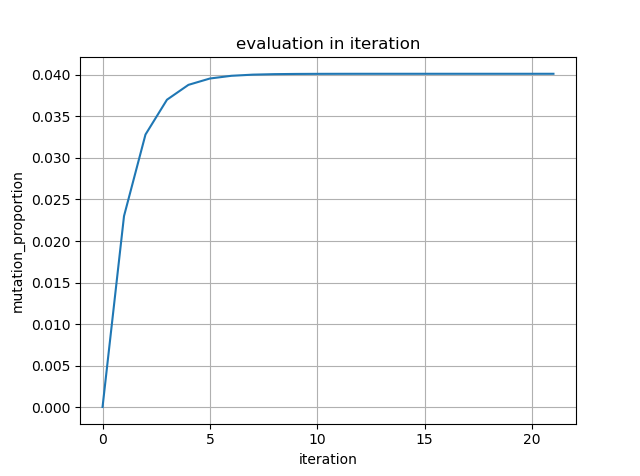
\includegraphics[width=0.7\textwidth]{Aufgabe_2c_2.png} 
\caption{Aufgabe2c 2} 
\label{Fig.main2} 
\end{figure}
%-------------------------------------------------------------------------------------------------------------3-------------------------------------------------------------------------------------------
\subsubsection*{3}
\begin{figure}[H] 
\centering 
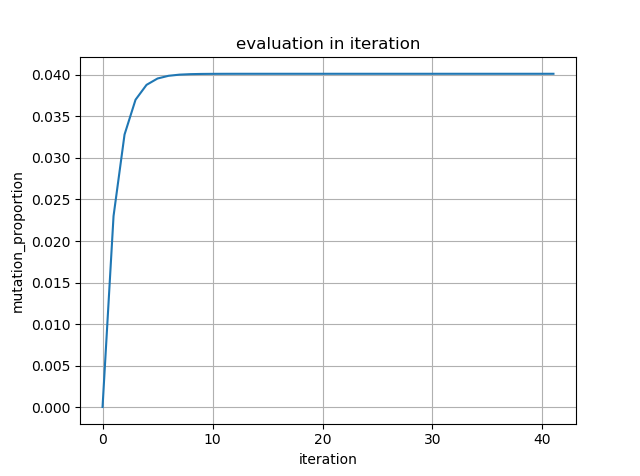
\includegraphics[width=0.7\textwidth]{Aufgabe_2c_3.png} 
\caption{Aufgabe2c 3} 
\label{Fig.main3}
\end{figure}
approximate at 5th step will culture contain stop to change mutation\\[20pt]
if 
\begin{equation}\notag
\begin{aligned}
45\%m+2.6\% \tilde{m}&=m \qquad with \tilde{m} = (1-m)\\
&\Rightarrow m \approx 4.01\% \\
\end{aligned}
\end{equation}
$\Rightarrow$
Evaluation proves get stable probability
\newpage
%--------------------------------------------------------------------------------------------------------Task3---------------------------------------------------------------------------------------------
\section*{Task 3}
%-------------------------------------------------------------------------------------------------------3a-----------------------------------------------------------------------------------
\subsection*{3a}
$
h(p_i) = -log_2 P_i \\[15pt]
 \qquad h(p_{S_1}) = 5.6439 \qquad h(p_{S_2}) = 0.5778  \qquad h(p_{S_3}) = 2.1203  \qquad h(p_{S_4}) = 3.6439  
$
\\[15pt]
average informaiton : 
$
H_{(p)}=E[h_{(p)}]= \sum\limits_{i=1}^{n}p_i h_{(p_i)}=1.2792 bit
$
\\[15pt]
In general: max: $log_2(4)=2bit$\\[15pt]
Uniform distribution is required to achieve this\\[15pt]
%----------------------------------------------------------------------------------------------------------3b---------------------------------------------------------------------------------------
\subsection*{3b}
%----------------------------------------------------------------------------------------------------------------1------------------------------------------------------------------------------
\subsubsection*{1}
additional condition :
$
1=\sum\limits_{i=1}^{4}p_i\qquad with 1\geq p_i \geq 0 \qquad i = 1,2,3 or 4
$
%-----------------------------------------------------------------------------------------------------------2------------------------------------------------------------------------------------------
\subsubsection*{2}
Cost function :(here Entrope with unit "nat" not unit "bit")\\
\begin{equation}\notag
\begin{aligned}
max_p \quad H(p)&=-\sum\limits_{i=1}^{4}p_i ln(p_i)\\
s.t. \quad t_1(p) &= \sum\limits_{i=1}^{4}2p_i \cdot i -6 = 0\\
t_2(p)&=\sum\limits_{i=1}^{4}p_i-1=0\\
Lagrangian\quad funciton \qquad L(\uline{p},\lambda) &= -\sum\limits_{i=1}^{4}p_i ln(p_i) + \lambda_1(\sum\limits_{i=1}^{4}2p_i \cdot i -6)+ \lambda_2(\sum\limits_{i=1}^{4}p_i-1)
\end{aligned}
\end{equation}
%-------------------------------------------------------------------------------------------------------------3-----------------------------------------------------------------------------------
\subsubsection*{3}
\begin{equation}\notag
\begin{aligned}
\frac{\partial L}{\partial \lambda_1}&=\sum\limits_{i=1}^{4}2p_i \cdot i -6\\
\frac{\partial L}{\partial \lambda_2}&=\sum\limits_{i=1}^{4}p_i -1 \Rightarrow monotone\quad increasing
\end{aligned}
\end{equation}
\uline{p} is correlative with $\frac{\partial L}{\partial \lambda_1}  \Rightarrow$ very hard to analytically solve
%-------------------------------------------------------------------------------------------------------------4---------------------------------------------------------------------------------
\subsubsection*{4}
Dual Formulation\\
\begin{equation}\notag
\begin{aligned}
max_p \quad H(p)&=-\sum\limits_{i=1}^{4}p_i ln(p_i)\\
s.t. \quad t_1(p) &= \sum\limits_{i=1}^{4}2p_i \cdot i -6 = 0\\
t_2(p)&=\sum\limits_{i=1}^{4}p_i-1=0\\
1)\qquad &L(\uline{p},\lambda) = -\sum\limits_{i=1}^{4}p_i h(p_i) + \lambda_1(\sum\limits_{i=1}^{4}2p_i \cdot i -6)+ \lambda_2(\sum\limits_{i=1}^{4}p_i-1)\\
2)\qquad &\frac{\partial L}{\partial \lambda_i} = -ln(p_i)+1+\lambda_1 \cdot 2i + \lambda_2 =0\\
 &\Rightarrow ln(p_i)= 1+\lambda_1 \cdot 2i + \lambda_2\\
&p^{*}_{i}= e^{(1+\lambda_1 \cdot 2i + \lambda_2)}\\
3) \qquad  &replace \quad p^{*}_{i}  \quad  in  \quad L(\uline{p},\lambda)\\
\Rightarrow G(\lambda) &=  -\sum\limits_{i=1}^{4} (1+\lambda_1 \cdot 2i + \lambda_2)\cdot e^{(1+\lambda_1 \cdot 2i + \lambda_2)}\\
&\quad + (\sum\limits_{i=1}^{4}2\lambda_1\cdot e^{(1+\lambda_1 \cdot 2i + \lambda_2)}-6\lambda_1)+(\sum\limits_{i=1}^{4}\lambda_2\cdot e^{(1+\lambda_1 \cdot 2i + \lambda_2)}-\lambda_2)\\
&= -\sum\limits_{i=1}^{4}  e^{(1+\lambda_1 \cdot 2i + \lambda_2)}-6\lambda_1-\lambda_2
\end{aligned}
\end{equation}
assume that $G(x)$ is a convex function\\
$$ 
\left\{
\begin{aligned}
\frac{\partial G}{\partial \lambda_1} & = & -\sum\limits_{i=1}^{4} 2i\cdot e^{(1+\lambda_1 \cdot 2i + \lambda_2)}-6&=&0 \\
\frac{\partial G}{\partial \lambda_2} & = & -\sum\limits_{i=1}^{4}\cdot e^{(1+\lambda_1 \cdot 2i + \lambda_2)}-1&=&0 \\
\end{aligned}
\right.
$$
$
\Rightarrow \lambda_1=solve_1 \qquad \lambda_2=solve_2
$
\\
\begin{figure}[H] 
\centering 
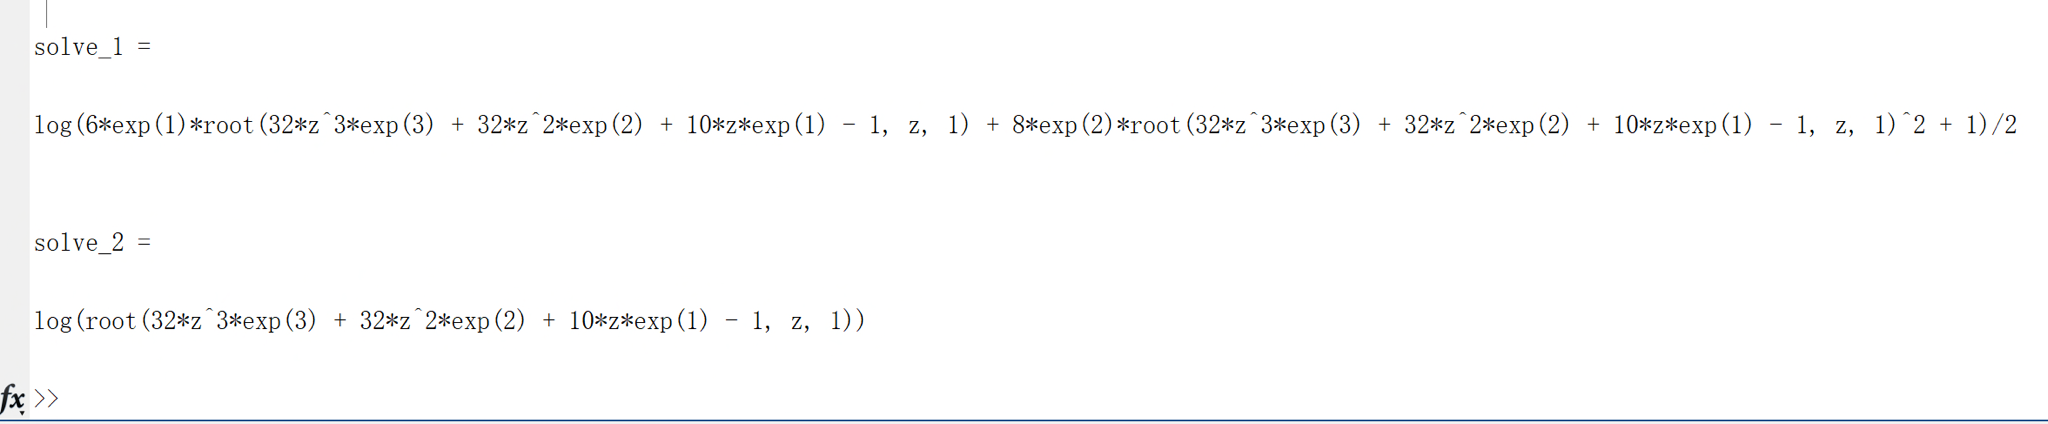
\includegraphics[width=1\textwidth]{Aufgabe3 4b.png} 
\caption{Aufgabe3b 4} 
\label{Fig.main4}
\end{figure}
%-------------------------------------------------------------------------------------------------5------------------------------------------------------------------------------------------
\subsubsection*{5}
Gradient descent is based on the observation that if the multi-variable function 
${\displaystyle F(\mathbf {x} )}$
is defined and differentiable in a neighborhood of a point 
${\displaystyle \mathbf {a} }$ , 
then 
${\displaystyle F(\mathbf {x} )}$
 decreases fastest if one goes from 
${\displaystyle \mathbf {a} }$
 in the direction of the negative gradient of 
${\displaystyle F}$
 at ${\displaystyle \mathbf {a} ,-\nabla F(\mathbf {a} )}$. 
It follows that, if\\
\begin{equation}\notag
\begin{aligned}
{\displaystyle \mathbf {a} _{n+1}=\mathbf {a} _{n}-\gamma \nabla F(\mathbf {a} _{n})}
\end{aligned}
\end{equation}
for 
${\displaystyle \gamma \in \mathbb {R} _{+}}$
 small enough, then 
${\displaystyle F(\mathbf {a_{n}} )\geq F(\mathbf {a_{n+1}} )}$.
 In other words, the term ${\displaystyle \gamma \nabla F(\mathbf {a} )}$
is subtracted from 
${\displaystyle \mathbf {a} }$
 because we want to move against the gradient, toward the local minimum. With this observation in mind, one starts with a guess 
${\displaystyle \mathbf {x} _{0}}$
 for a local minimum of 
${\displaystyle F}$, 
and considers the sequence 
${\displaystyle \mathbf {x} _{0},\mathbf {x} _{1},\mathbf {x} _{2},\ldots }$
 such that\\
\begin{equation}\notag
\begin{aligned}
\mathbf {x} _{n+1}=\mathbf {x} _{n}-\gamma _{n}\nabla F(\mathbf {x} _{n}),\ n\geq 0.
\end{aligned}
\end{equation}
We have a monotonic sequence\\
\begin{equation}\notag
\begin{aligned}
{\displaystyle F(\mathbf {x} _{0})\geq F(\mathbf {x} _{1})\geq F(\mathbf {x} _{2})\geq \cdots ,}
\end{aligned}
\end{equation}
so hopefully the sequence 
${\displaystyle (\mathbf {x} _{n})}$
 converges to the desired local minimum. Note that the value of the step size 
${\displaystyle \gamma }$
  is allowed to change at every iteration. With certain assumptions on the function 
${\displaystyle F}$
 (for example, 
${\displaystyle F}$ 
convex and 
${\displaystyle \nabla F}$
 Lipschitz) and particular choices of 
${\displaystyle \gamma }$ (e.g., chosen either via a line search that satisfies the Wolfe conditions, or the Barzilai–Borwein method shown as following),\\
\begin{equation}\notag
\begin{aligned}
{\displaystyle \gamma _{n}={\frac {\left|\left(\mathbf {x} _{n}-\mathbf {x} _{n-1}\right)^{T}\left[\nabla F(\mathbf {x} _{n})-\nabla F(\mathbf {x} _{n-1})\right]\right|}{\left\|\nabla F(\mathbf {x} _{n})-\nabla F(\mathbf {x} _{n-1})\right\|^{2}}}}
\end{aligned}
\end{equation}
convergence to a local minimum can be guaranteed. When the function
 ${\displaystyle F}$ 
is convex, all local minima are also global minima, so in this case gradient descent can converge to the global solution.\\[10pt]
This process is illustrated in the adjacent picture. Here 
${\displaystyle F}$
 is assumed to be defined on the plane, and that its graph has a bowl shape. The blue curves are the contour lines, that is, the regions on which the value of 
${\displaystyle F}$ 
is constant. A red arrow originating at a point shows the direction of the negative gradient at that point. Note that the (negative) gradient at a point is orthogonal to the contour line going through that point. We see that gradient descent leads us to the bottom of the bowl, that is, to the point where the value of the function 
${\displaystyle F}$ 
is minimal.\\
\begin{figure}[H] 
\centering 
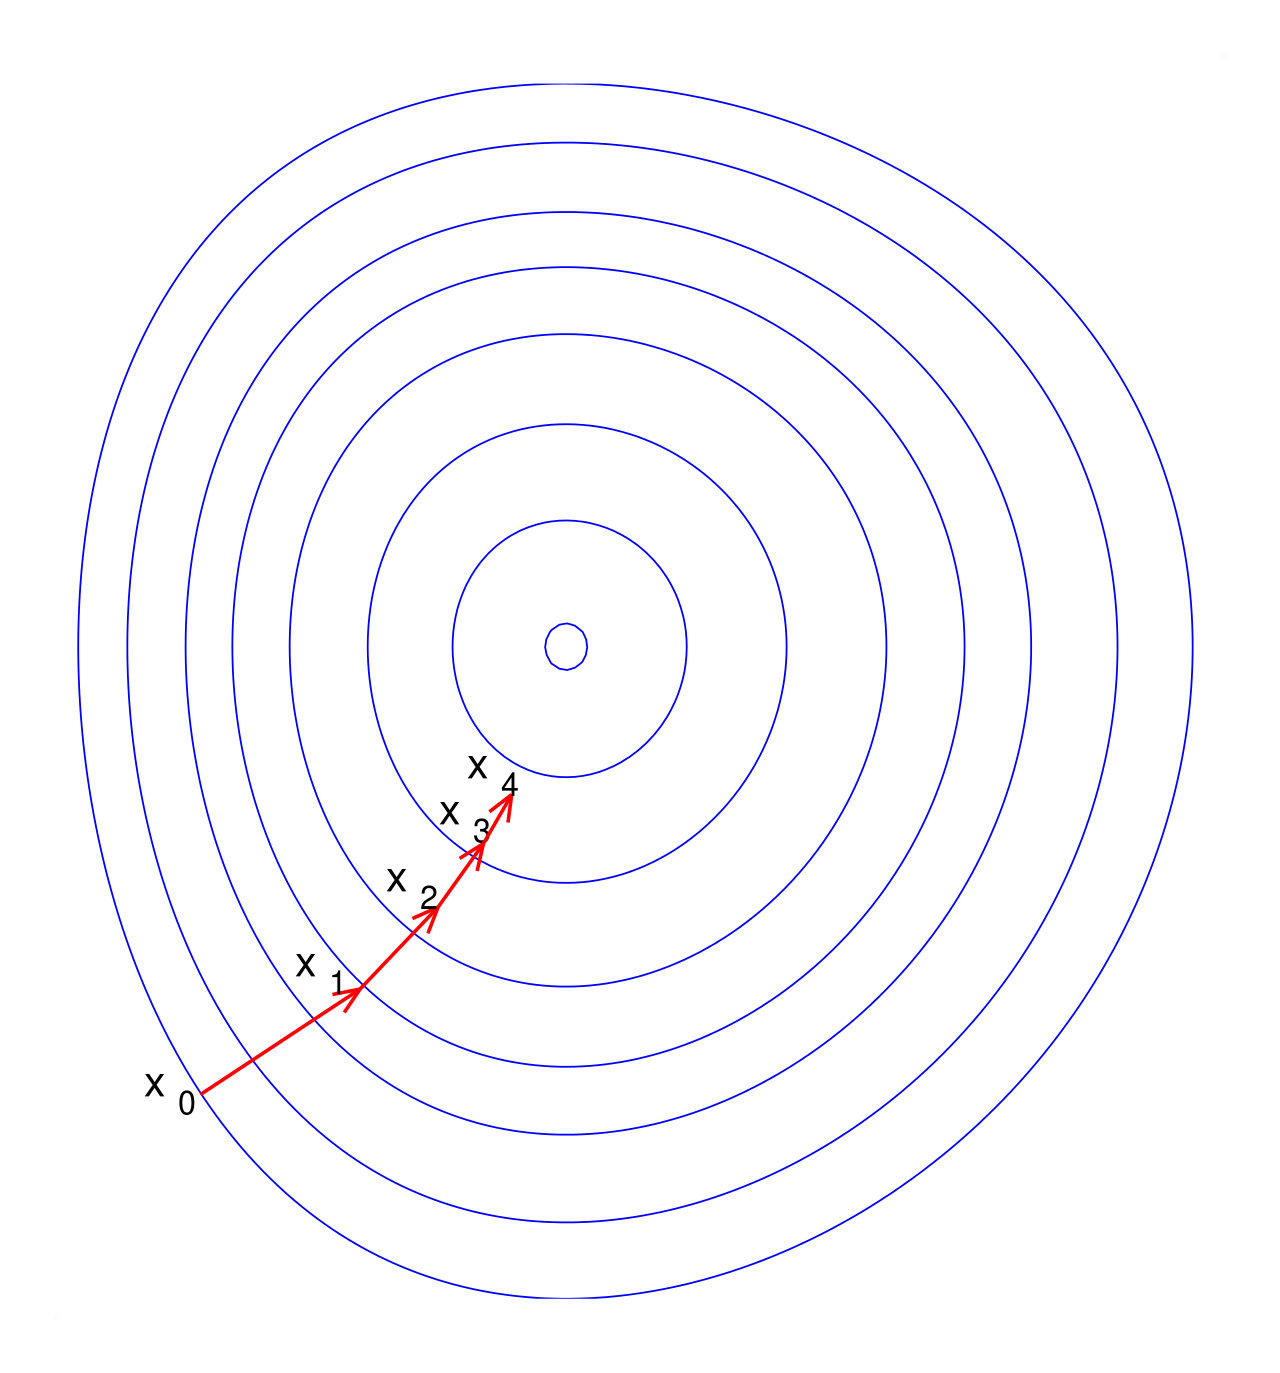
\includegraphics[width=0.3\textwidth]{Gradient_descent.svg.png} 
\caption{Gradient descent} 
\label{Fig.main5}
\end{figure}
%------------------------------------------------------------------------------------------------------------------------3c----------------------------------------------------------------
\subsubsection*{3c}
\begin{lstlisting}
# -*- coding: utf-8 -*-

import numpy as np
import matplotlib.pyplot as plt


def benchmark_function(array_x=np.random.random((20, 1))):
    """
    evaluate Rosenbrock's function under array_x
    :param array_x: [array], multidimensional variable (default value: np.random.random((20, 1)))
    :return:
    cost [float], the value of Rosenbrock's function
    """
    # initial list of intermediate variables
    value_list = []

    # compute
    for i in range(array_x.shape[0]-1):
        f_x = 100*(array_x[i+1] - array_x[i]**2)**2 + (array_x[i] - 1)**2
        value_list.append(f_x)

    return sum(value_list)


def gradient_descent(array_x):
    """
    compute gradient  in Rosenbrock's function
    :param array_x: [array], input array
    :return:
    [array], the gradient matrix,  size(n x 1)
    """
    # initial list of intermediate variables
    row_list = []

    # compute
    for i in range(array_x.shape[0]):
        # initial for each for
        row = []
        for j in range(array_x.shape[0] - 1):
            if i == j:
                d_fx = 200*(array_x[i+1] - array_x[i]**2)*(-2*array_x[i]) + 2*array_x[i]
                row.append(float(d_fx))
            elif i == j+1:
                d_fx = 200*(array_x[i] - array_x[i-1]**2)
                row.append(float(d_fx))
            else:
                row.append(0)
        row_list.append(row)

    # convert list to array, size(n-1 x n)
    gradient_matrix = np.array(row_list)

    # merge matrix in vector
    gradient_vector = np.sum(gradient_matrix, axis=1, dtype='float64').reshape(array_x.shape[0], 1)

    return gradient_vector


def var_updating(array_x, alpha=1e-3, epoch=500):
    """
    update variable with gradient descent in iteration
    :param array_x: [array], initial variable, size(n x 1)
    :param alpha: [float], learning rate (default value: 1e-3)
    :param epoch: [int] , time of iteration
    :return:
    """
    # initial cost record
    cost_hist = [benchmark_function(array_x)]

    # initial iteration record
    iteration = 0

    for i in range(epoch):
        # compute gradient
        gradient_vector = gradient_descent(array_x)

        # update array
        array_x = array_x - alpha * gradient_vector

        # compute cost
        cost = benchmark_function(array_x)

        cost_hist.append(cost)

        # assign necessary iteration
        if i> 10 and iteration == 0 and \
                (cost_hist[i-1]-cost_hist[i])/cost_hist[i] <= 1e-80:
            iteration = i
            continue

    return cost_hist, iteration


def plot_cost(cost_hist, alpha=1e-3, iteration=500):
    """
    plot evaluation history of bacterium with mutation
    :param cost_hist: , the record of evaluation history
    :param alpha: [float], learning rate (default value: 1e-3)
    :return:
    """
    # assign plot data in dict form
    data = {"cost": cost_hist,
            "iteration": np.linspace(0, len(cost_hist), len(cost_hist), dtype=np.int16)}

    # initial figure
    plt.plot("iteration", "cost", data=data, label=f'alpha = {alpha}, iteration = {iteration}')
    plt.grid()
    plt.xlabel("iteration")
    plt.ylabel("Rosenbrock's function")
    plt.title("learning curve")

    return plt


if __name__ == '__main__':
    # set random seed
    np.random.seed(233)

    # set search space
    candidate_alpha = np.logspace(-10, -1, 10)

    plt.figure(1)

    for alpha in candidate_alpha:
        array_x = np.random.random((20, 1))
        hist, iteration = var_updating(array_x)
        plt = plot_cost(hist, alpha=alpha, iteration=iteration)

    plt.legend()
    plt.grid()
    plt.show()
\end{lstlisting}
\begin{figure}[H] 
\centering 
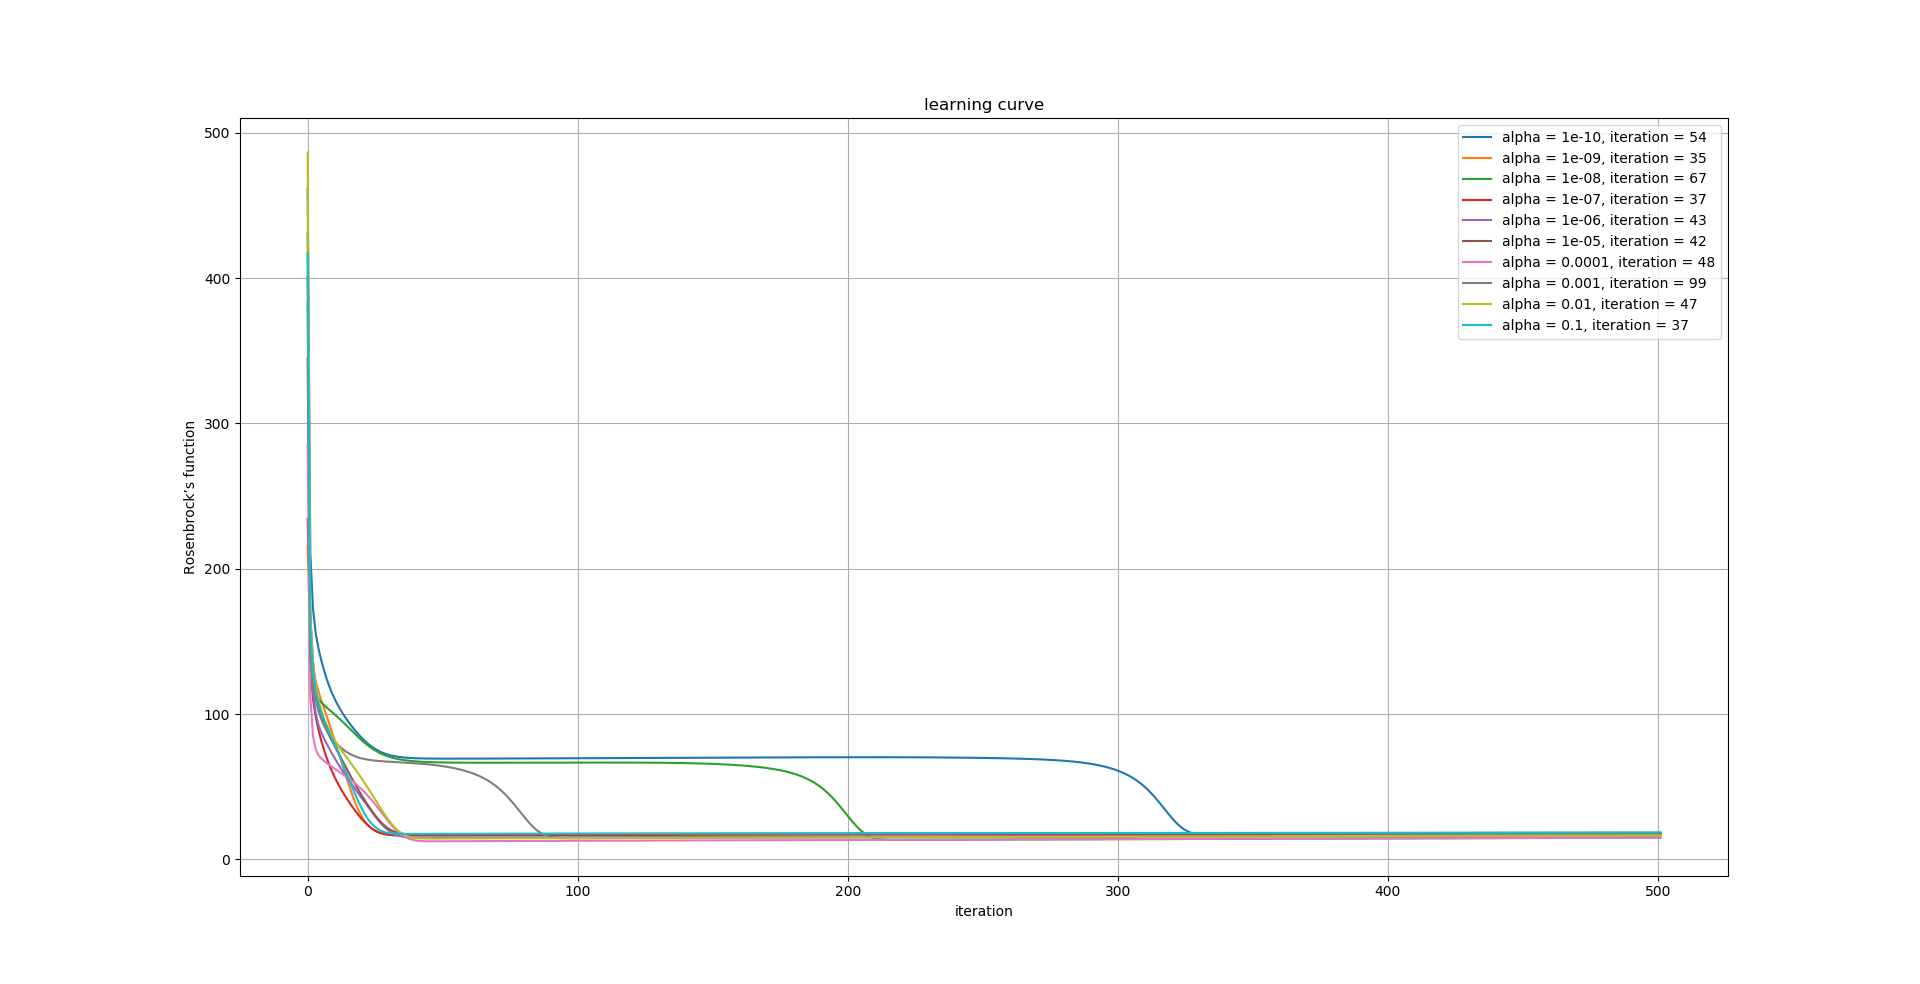
\includegraphics[width=1\textwidth]{Aufgabe_3c.png} 
\caption{Aufgabe3c} 
\label{Fig.main6}
\end{figure}
\newpage
%------------------------------------------------------------------------------------------------------------------------------3d-------------------------------------------------------------------------
\subsubsection*{3d}
%------------------------------------------------------------------------------------------------------------------------------1-------------------------------------------------------------------------
\subsubsection*{1}
Vanilla means standard, usual, or unmodified version of something. Vanilla gradient descent means the basic gradient descent algorithm without any bells or whistles.\\
There are many variants on gradient descent. In usual gradient descent (also known as batch gradient descent or vanilla gradient descent), the gradient is computed as the average of the gradient of each datapoint.\\
\begin{equation}\notag
\begin{aligned}
\nabla f = \frac{1}{n}\sum_i \nabla \text{loss}(x_i)
\end{aligned}
\end{equation}
pros:\\
great for convex, or relatively smooth error manifolds\\
cons:\\
too computationally expensive for not that much of a gain\\[15pt]
In stochastic gradient descent with a batch size of one, we might estimate the gradient as
\begin{equation}\notag
\begin{aligned}
\nabla f \approx \nabla \text{loss}(x^*)
\end{aligned}
\end{equation}
, where $x^*$ is randomly sampled from our entire dataset. It is a variant of normal gradient descent, so it wouldn't be vanilla gradient descent\\
pros:\\
computationally a lot faster\\
cons:\\
single samples are really noisy\\
The trade off between vanilla gradient descend and stochastic gradient descend is that is called mini-batch gradient descend.In this method,the objective function is computed over a small batch of samples. The size of batch is much smaller than the size of samples in the training set.\\
pros:\\
small enough to avoid some of the poor local minima, but large enough that it doesn't avoid the global minima or better-performing local minima\\
cons:\\
not easy to find a suitable batch size\\
%------------------------------------------------------------------------------------------------------------------------2---------------------------------------------------------------------------
\subsubsection*{2}
Gradient Descent with Momentum considers the past gradients to smooth out the update. It computes an exponentially weighted average of your gradients, and then use that gradient to update the weights instead. It works faster than the standard gradient descent algorithm.\\
It is not always useful \\
%----------------------------------------------------------------------------------------------------------------------暂时没太知道啥时候不行----------------------------------------------------------------
\end{document}